%%%%%%%%%%%%%%%%%%%%%%%%%%%%%%%%%%%%%%%%%%%%%%%%%%%%%%%%%%%%%%%
%% OXFORD THESIS TEMPLATE

% Use this template to produce a standard thesis that meets the Oxford University requirements for DPhil submission
%
% Originally by Keith A. Gillow (gillow@maths.ox.ac.uk), 1997
% Modified by Sam Evans (sam@samuelevansresearch.org), 2007
% Modified by John McManigle (john@oxfordechoes.com), 2015
%
% This version Copyright (c) 2015-2017 John McManigle
%
% Broad permissions are granted to use, modify, and distribute this software
% as specified in the MIT License included in this distribution's LICENSE file.
%

% I've (John) tried to comment this file extensively, so read through it to see how to use the various options.  Remember
% that in LaTeX, any line starting with a % is NOT executed.  Several places below, you have a choice of which line to use
% out of multiple options (eg draft vs final, for PDF vs for binding, etc.)  When you pick one, add a % to the beginning of
% the lines you don't want.


%%%%% CHOOSE PAGE LAYOUT
% The most common choices should be below.  You can also do other things, like replacing "a4paper" with "letterpaper", etc.

% This one will format for two-sided binding (ie left and right pages have mirror margins; blank pages inserted where needed):
% \documentclass[a4paper,twoside]{ociamthesis}
% This one will format for one-sided binding (ie left margin > right margin; no extra blank pages):
%\documentclass[a4paper]{ociamthesis}
% This one will format for PDF output (ie equal margins, no extra blank pages):
\documentclass[a4paper,nobind]{ociamthesis} 



%%%%% SELECT YOUR DRAFT OPTIONS
% Three options going on here; use in any combination.  But remember to turn the first two off before
% generating a PDF to send to the printer!

% This adds a "DRAFT" footer to every normal page.  (The first page of each chapter is not a "normal" page.)
\fancyfoot[C]{\emph{Version from \today}}  

% This highlights (in blue) corrections marked with (for words) \mccorrect{blah} or (for whole
% paragraphs) \begin{mccorrection} . . . \end{mccorrection}.  This can be useful for sending a PDF of
% your corrected thesis to your examiners for review.  Turn it off, and the blue disappears.
\correctionstrue


%%%%% BIBLIOGRAPHY SETUP
% Note that your bibliography will require some tweaking depending on your department, preferred format, etc.
% The options included below are just very basic "sciencey" and "humanitiesey" options to get started.
% If you've not used LaTeX before, I recommend reading a little about biblatex/biber and getting started with it.
% If you're already a LaTeX pro and are used to natbib or something, modify as necessary.
% Either way, you'll have to choose and configure an appropriate bibliography format...

% The science-type option: numerical in-text citation with references in order of appearance.
\usepackage[style=numeric-comp, sorting=none, backend=biber, doi=false, isbn=false]{biblatex}
\newcommand*{\bibtitle}{References}

% The humanities-type option: author-year in-text citation with an alphabetical works cited.
%\usepackage[style=authoryear, sorting=nyt, backend=biber, maxcitenames=2, useprefix, doi=false, isbn=false]{biblatex}
%\newcommand*{\bibtitle}{Works Cited}

% This makes the bibliography left-aligned (not 'justified') and slightly smaller font.
\renewcommand*{\bibfont}{\raggedright\small}

% Change this to the name of your .bib file (usually exported from a citation manager like Zotero or EndNote).
\addbibresource{references.bib}


% Uncomment this if you want equation numbers per section (2.3.12), instead of per chapter (2.18):
%\numberwithin{equation}{subsection}



%%%%% THESIS / TITLE PAGE INFORMATION
% Everybody needs to complete the following:
\title{Suitably impressive thesis title}
\author{Your Name}
\college{Your College}

% Master's candidates who require the alternate title page (with candidate number and word count)
% must also un-comment and complete the following three lines:
%\masterssubmissiontrue
%\candidateno{933516}
%\wordcount{28,815}

% Uncomment the following line if your degree also includes exams (eg most masters):
%\renewcommand{\submittedtext}{Submitted in partial completion of the}
% Your full degree name.  (But remember that DPhils aren't "in" anything.  They're just DPhils.)
\degree{Doctor of Philosophy}
% Term and year of submission, or date if your board requires (eg most masters)
\degreedate{Michaelmas 2014}


%%%%% YOUR OWN PERSONAL MACROS
% This is a good place to dump your own LaTeX macros as they come up.
\usepackage{graphicx}

% To make text superscripts shortcuts
	\renewcommand{\th}{\textsuperscript{th}} % ex: I won 4\th place
	\newcommand{\nd}{\textsuperscript{nd}}
	\renewcommand{\st}{\textsuperscript{st}}
	\newcommand{\rd}{\textsuperscript{rd}}

%%%%% THE ACTUAL DOCUMENT STARTS HERE
\begin{document}



%%%%% CHOOSE YOUR LINE SPACING HERE
% This is the official option.  Use it for your submission copy and library copy:
\setlength{\textbaselineskip}{22pt plus2pt}
% This is closer spacing (about 1.5-spaced) that you might prefer for your personal copies:
%\setlength{\textbaselineskip}{18pt plus2pt minus1pt}

% You can set the spacing here for the roman-numbered pages (acknowledgements, table of contents, etc.)
\setlength{\frontmatterbaselineskip}{17pt plus1pt minus1pt}

% Leave this line alone; it gets things started for the real document.
\setlength{\baselineskip}{\textbaselineskip}


%%%%% CHOOSE YOUR SECTION NUMBERING DEPTH HERE
% You have two choices.  First, how far down are sections numbered?  (Below that, they're named but
% don't get numbers.)  Second, what level of section appears in the table of contents?  These don't have
% to match: you can have numbered sections that don't show up in the ToC, or unnumbered sections that
% do.  Throughout, 0 = chapter; 1 = section; 2 = subsection; 3 = subsubsection, 4 = paragraph...

% The level that gets a number:
\setcounter{secnumdepth}{2}
% The level that shows up in the ToC:
\setcounter{tocdepth}{2}


%%%%% ABSTRACT SEPARATE
% This is used to create the separate, one-page abstract that you are required to hand into the Exam
% Schools.  You can comment it out to generate a PDF for printing or whatnot.
\begin{abstractseparate}
	%Move 1: Background to the Dissertation
%Move 2: Statement of the Problem/Gap in the Research
%Move 3: Purpose of the Dissertation
%Move 4: Work carried out/Methods
%Move 5: Results
%Move 6: Conclusions/Implications
%Move 7: Contribution of the Dissertation 

Alternative Splicing (AS) is a fundamental part of gene expression and its misregulation has been associated with up to 20\% of all diseases, yet the regulatory mechanisms influencing it are still poorly understood. Better understanding of AS is in part driven by computational models which predict AS behaviour based on sequence information. 

Here, we show that a dataset which was previously widely used for the quantification of AS is systematically biased, calling the meaningfulness of results using this dataset into question. To this end, we construct three new datasets, each based on a different processing method, and show that only of them provides high enough data quality for our task. We develop a new Deep Learning model which is the first to introduce the Attention mechanism to AS prediction. Evaluating our newly proposed model, we reimplement two models from the literature and find that it outperforms the previous state-of-the-art by 15\%. Finally, we interpret our model and show that it attends to biologically plausible motifs. 
Thus, our work shows that previous results have been based on systematically biased data,
% may not be as meaningful
provides better datasets upon which future work can build and introduces a new state-of-the-art model. 

%maybe: introduce splicing codes as those models which do the thing
%maybe: say that my model is named RASC % Create an abstract.tex file in the 'text' folder for your abstract.
\end{abstractseparate}


% JEM: Pages are roman numbered from here, though page numbers are invisible until ToC.  This is in
% keeping with most typesetting conventions.
\begin{romanpages}

% Title page is created here
\maketitle

%%%%% DEDICATION -- If you'd like one, un-comment the following.
%\begin{dedication}
%This thesis is dedicated to\\
%someone\\
%for some special reason\\
%\end{dedication}

%%%%% ACKNOWLEDGEMENTS -- Nothing to do here except comment out if you don't want it.
\begin{acknowledgements}
 	\subsection*{Personal}

This is where you thank your advisor, colleagues, and family and friends.

Lorem ipsum dolor sit amet, consectetur adipiscing elit. Vestibulum feugiat et est at accumsan. Praesent sed elit mattis, congue mi sed, porta ipsum. In non ullamcorper lacus. Quisque volutpat tempus ligula ac ultricies. Nam sed erat feugiat, elementum dolor sed, elementum neque. Aliquam eu iaculis est, a sollicitudin augue. Cras id lorem vel purus posuere tempor. Proin tincidunt, sapien non dictum aliquam, ex odio ornare mauris, ultrices viverra nisi magna in lacus. Fusce aliquet molestie massa, ut fringilla purus rutrum consectetur. Nam non nunc tincidunt, rutrum dui sit amet, ornare nunc. Donec cursus tortor vel odio molestie dignissim. Vivamus id mi erat. Duis porttitor diam tempor rutrum porttitor. Lorem ipsum dolor sit amet, consectetur adipiscing elit. Sed condimentum venenatis consectetur. Lorem ipsum dolor sit amet, consectetur adipiscing elit.

Aenean sit amet lectus nec tellus viverra ultrices vitae commodo nunc. Mauris at maximus arcu. Aliquam varius congue orci et ultrices. In non ipsum vel est scelerisque efficitur in at augue. Nullam rhoncus orci velit. Duis ultricies accumsan feugiat. Etiam consectetur ornare velit et eleifend.

Suspendisse sed enim lacinia, pharetra neque ac, ultricies urna. Phasellus sit amet cursus purus. Quisque non odio libero. Etiam iaculis odio a ex volutpat, eget pulvinar augue mollis. Mauris nibh lorem, mollis quis semper quis, consequat nec metus. Etiam dolor mi, cursus a ipsum aliquam, eleifend venenatis ipsum. Maecenas tempus, nibh eget scelerisque feugiat, leo nibh lobortis diam, id laoreet purus dolor eu mauris. Pellentesque habitant morbi tristique senectus et netus et malesuada fames ac turpis egestas. Nulla eget tortor eu arcu sagittis euismod fermentum id neque. In sit amet justo ligula. Donec rutrum ex a aliquet egestas.

\subsection*{Institutional}

If you want to separate out your thanks for funding and institutional support, I don't think there's any rule against it.  Of course, you could also just remove the subsections and do one big traditional acknowledgement section.

Lorem ipsum dolor sit amet, consectetur adipiscing elit. Ut luctus tempor ex at pretium. Sed varius, mauris at dapibus lobortis, elit purus tempor neque, facilisis sollicitudin felis nunc a urna. Morbi mattis ante non augue blandit pulvinar. Quisque nec euismod mauris. Nulla et tellus eu nibh auctor malesuada quis imperdiet quam. Sed eget tincidunt velit. Cras molestie sem ipsum, at faucibus quam mattis vel. Quisque vel placerat orci, id tempor urna. Vivamus mollis, neque in aliquam consequat, dui sem volutpat lorem, sit amet tempor ipsum felis eget ante. Integer lacinia nulla vitae felis vulputate, at tincidunt ligula maximus. Aenean venenatis dolor ante, euismod ultrices nibh mollis ac. Ut malesuada aliquam urna, ac interdum magna malesuada posuere.
\end{acknowledgements}

%%%%% ABSTRACT -- Nothing to do here except comment out if you don't want it.
\begin{abstract}
	%Move 1: Background to the Dissertation
%Move 2: Statement of the Problem/Gap in the Research
%Move 3: Purpose of the Dissertation
%Move 4: Work carried out/Methods
%Move 5: Results
%Move 6: Conclusions/Implications
%Move 7: Contribution of the Dissertation 

Alternative Splicing (AS) is a fundamental part of gene expression and its misregulation has been associated with up to 20\% of all diseases, yet the regulatory mechanisms influencing it are still poorly understood. Better understanding of AS is in part driven by computational models which predict AS behaviour based on sequence information. 

Here, we show that a dataset which was previously widely used for the quantification of AS is systematically biased, calling the meaningfulness of results using this dataset into question. To this end, we construct three new datasets, each based on a different processing method, and show that only of them provides high enough data quality for our task. We develop a new Deep Learning model which is the first to introduce the Attention mechanism to AS prediction. Evaluating our newly proposed model, we reimplement two models from the literature and find that it outperforms the previous state-of-the-art by 15\%. Finally, we interpret our model and show that it attends to biologically plausible motifs. 
Thus, our work shows that previous results have been based on systematically biased data,
% may not be as meaningful
provides better datasets upon which future work can build and introduces a new state-of-the-art model. 

%maybe: introduce splicing codes as those models which do the thing
%maybe: say that my model is named RASC
\end{abstract}

%%%%% MINI TABLES
% This lays the groundwork for per-chapter, mini tables of contents.  Comment the following line
% (and remove \minitoc from the chapter files) if you don't want this.  Un-comment either of the
% next two lines if you want a per-chapter list of figures or tables.
\dominitoc % include a mini table of contents
%\dominilof  % include a mini list of figures
%\dominilot  % include a mini list of tables

% This aligns the bottom of the text of each page.  It generally makes things look better.
\flushbottom

% This is where the whole-document ToC appears:
\tableofcontents

\listoffigures
	\mtcaddchapter
% \mtcaddchapter is needed when adding a non-chapter (but chapter-like) entity to avoid confusing minitoc

% Uncomment to generate a list of tables:
%\listoftables
%	\mtcaddchapter
fuvr
%%%%% LIST OF ABBREVIATIONS
% This example includes a list of abbreviations.  Look at text/abbreviations.tex to see how that file is
% formatted.  The template can handle any kind of list though, so this might be a good place for a
% glossary, etc.
% First parameter can be changed eg to "Glossary" or something.
% Second parameter is the max length of bold terms.
%To keep this glossary useful, we mainly focus on abbreviations specific to our domain and don't list very common abbrevations (such as NLP - Natural Language Processing).
\begin{mclistof}{Glossary}{3.2cm}

%\item[NLP] Natural Language Processing
%\item[CV] Computer Vision
\item[Splicing] Process by which a pre-mRNA is converted to a mature mRNA or the actual act of cutting out genomic sequences in that process itself.
\item[Exon] Genomic sequence which is typically kept from the pre-mRNA during splicing.
\item[Intron] Genomic sequence which is typically removed from the pre-mRNA during splicing.
\item[PSI] Percent-spliced in, in what proportions of transcript a specific exon (or junction) is contained in the mature mRNA.
%\item[MLP] Multi-layer perceptron
%\item[w2v] word2vec algorithm
%\item[D2V] Either the algorithm document2vector, or the specific model based on this algorithm.
\item[EST] Expressed sequence tag, a short cDNA sequence used in older sequencing techniques.
\item[GTEx] Genotype-Tissue Expression project, they provide a large repository of sequencing data which we use.

\item[iPSC] induced pluripotent stem cells, mature cells which have been reprogrammed to again become pluripotent (undetermined).
\item[HipSci] Human Induced Pluripotent Stem Cell Initiative, a repository of iPSC-based data which we use.

%\item[ROC] Receiver Operating Curve
%\item[AUC] Area under ROC curve
%\item[Seq2seq] Sequence-to-sequence learning, a framework often used in MT.
%\item[MT] Machine Translation
%\item[RNN] Recurrent Neural Network
%\item[CNN] Convolutional Neural Network
\item[DSC] Deep Splicing Code, a model used for constitutive exon classification.



\end{mclistof} 


% The Roman pages, like the Roman Empire, must come to its inevitable close.
\end{romanpages}


%%%%% CHAPTERS
% Add or remove any chapters you'd like here, by file name (excluding '.tex'):
\flushbottom
\begin{savequote}[8cm]
\textlatin{Neque porro quisquam est qui dolorem ipsum quia dolor sit amet, consectetur, adipisci velit...}

There is no one who loves pain itself, who seeks after it and wants to have it, simply because it is pain...
  \qauthor{--- Cicero's \textit{de Finibus Bonorum et Malorum}}
\end{savequote}

\chapter{\label{ch:1-intro}Introduction} 

%\minitoc

"Why genes in pieces?" -- can put this citation at the top and start with related story
\section{Motivation}


\section{Contribution}




\begin{savequote}[8cm]
Alles Gescheite ist schon gedacht worden.\\
Man muss nur versuchen, es noch einmal zu denken.

All intelligent thoughts have already been thought;\\
what is necessary is only to try to think them again.
  \qauthor{--- Johann Wolfgang von Goethe \cite{von_goethe_wilhelm_1829}}
\end{savequote}

\chapter{\label{ch:2-litreview}Background}

\minitoc

\section{Introduction}

This document introduction won't serve as a complete primer on \LaTeX.  There are plenty of those online, and googling your questions will often get you answers, especially from \url{http://tex.stackexchange.com}.

Instead, let's talk a little about a few of the features and packages lumped into this template situation.  The \verb|savequote| environment at the beginning of chapters can add some wittiness to your thesis.  If you don't like the quotes, just remove that block.

For when it comes time to do corrections, there are two useful commands here.  First, the \verb|mccorrect| command allows you to highlight a short correction \mccorrect{like this one}.  When the thesis is typeset normally, the correction will just appear as part of the text.  However, when you declare \verb|\correctionstrue| in the main \verb|Oxford_Thesis.tex| file, that correction will be highlighted in blue.  That might be useful for submitting a post-viva, corrected copy to your examiners so they can quickly verify you've completed the task.

\begin{mccorrection}
For larger chunks, like this paragraph or indeed entire figures, you can use the \verb|mccorrection| environment.  This environment highlights paragraph-sized and larger blocks with the same blue colour.
\end{mccorrection}

Read through the \verb|Oxford_Thesis.tex| file to see the various options for one- and two-sided printing, including or excluding the separate abstract page, and turning corrections and draft footer on or off, and the separate option to centre your text on the page (for PDF submission) or offset it (for binding).  There is also a separate option for master's degree submissions, which changes identifying information to candidate number and includes a word count.  (Unfortunately, \LaTeX has a hard time doing word counts automatically, so you'll have to enter the count manually if you require this.)

\section{Cardiac Imaging}\label{app:imaging}

Within months of Röntgen's discovery of the X-ray in \mccorrect{1895}\cite{gagliardi_rontgen_1996}, cardiac pathology was being investigated via non-invasive imaging \cite{gagliardi_cardiac_1996}.  Over the intervening years, cardiac imaging modalities and techniques have advanced significantly.  Clinically, cardiac imaging is used for two broad purposes: diagnosis of pathophysiology and guidance of interventional procedures.  These applications impose different requirements on imaging equipment, image acquisition time, computational complexity, spatial and temporal resolution, and tissue discrimination.  The common diagnostic and interventional cardiac imaging techniques in current clinical practice are reviewed below.  An accessible introduction to the physics of medical imaging can be found in Webb's \textit{Introduction to Biomedical Imaging} \cite{webb_introduction_2002}.  A comprehensive overview of the use of imaging in clinical cardiology is presented in Leeson's \textit{Cardiovascular Imaging} \cite{leeson_cardiovascular_2011}.

\subsection{Diagnostic Imaging}
\label{sub:diagnostic}

Beyond the chest X-ray (`plain film'), the key non-invasive imaging modalities in diagnostic cardiology are echocardiography, magnetic resonance imaging, and X-ray computed tomography, which are reviewed below.  Nuclear medicine, including positron emission tomography (PET) and single-photon emission computed tomography (SPECT), are not discussed here, as they do not play a role in the chapters to follow.

\subsubsection{Echocardiography}

\begin{figure}
\centering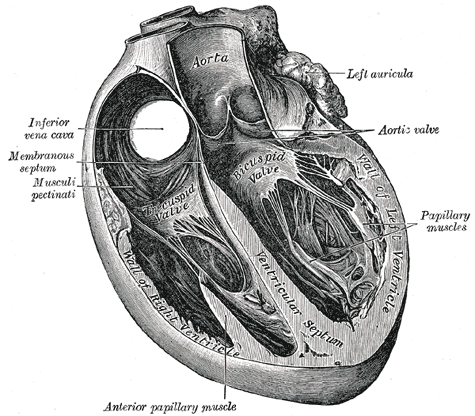
\includegraphics[width=0.7\textwidth]{figures/sample/Gray498.png} 
\caption[Four-chamber illustration of the human heart.]{Four-chamber illustration of the human heart.  Clockwise from upper-left: right atrium, left atrium, left ventricle, right ventricle.}
\label{fig:fourchamber}\end{figure}

The use of acoustic waves for medical diagnosis, inspired by naval sonar, was initially developed in the 1940s \cite{gagliardi_ultrasonography_1996}.  By 1954, the first clinically useful cardiac ultrasound -- examining motion of the mitral valve in stenosis -- was reported \cite{edler_ultrasonic_1957}.  These early scans were one-dimensional images (`A-mode'), sometimes repeated to generate a time axis (`M-mode').   The sector-scanning probe was developed in the 1970s \cite{bom_ultrasonic_1971,griffith_sector_1974}, leading to the `B-mode' that a modern cardiologist would recognise as an echocardiogram.



%% APPENDICES %% 
% Starts lettered appendices, adds a heading in table of contents, and adds a
%    page that just says "Appendices" to signal the end of your main text.
\startappendices
% Add or remove any appendices you'd like here:
\begin{savequote}[8cm]
\textlatin{Cor animalium, fundamentum e\longs t vitæ, princeps omnium, Microco\longs mi Sol, a quo omnis vegetatio dependet, vigor omnis \& robur emanat.}

The heart of animals is the foundation of their life, the sovereign of everything within them, the sun of their microcosm, that upon which all growth depends, from which all power proceeds.
  \qauthor{--- William Harvey %\cite{harvey_exercitatio_1628}
  }
\end{savequote}

\chapter{\label{app:appendix}Appendix}

\minitoc


\section{Accession Numbers of HipSci data} \label{app:hipsci_celllines}
The ENA Accession Numbers of the 25 biological replicates belonging to sensory neuron cell lines \cite{ipscneurons} are ERR177-: 
5544, 5551, 5552, 5554, 5594. 5595, 5596, 5598, 5600, 5601, 5631, 5634, 5637, 5638, 5640, 5641, 5643, 5644, 5684, 5685, 5686, 5687, 5688, 5689, 5693.
While all of these were used in MAJIQ Builder process (and thus contributed to the constitutive exons), only the sample with Accession Number ERR1775544 was used with the MAJIQ PSI step (and thus determined the alternatively spliced exons). 

The ENA Accession Numbers of the 20 biological replicates belonging to undifferentiated iPSC cell lines \cite{hipsci} are ERR-: 
914342, 946968, 946976, 946983, 946984, 946990, 946992, 946994, 947011, 1203463, 1243454, 1274914, 1274917, 1724696, 1724699, 1743789, 2039345, 2039336, 2278244 2278245.
Similarly, all of the above biological replicates were used in the MAJIQ Builder process. Only the samples with Accession Numbers ERR946992, ERR946984 (same cell type and donor as ERR946984, but different cell line), and ERR946968 (same cell type, but different donor) were used with MAJIQ PSI. 
%bezi1, 2 
%lexy 2
%25 biological replicates:
%ERR1775544 - 0 
%ERR1775551 - 1
%ERR1775552 - 2
%ERR1775553 - 3
%ERR1775554 - 4
%---
%ERR1775594 - 5
%ERR1775595 - 6
%ERR1775596 - 7
%ERR1775598 - 8
%ERR1775600 - 9
%ERR1775601 - 10
%--- 
%ERR1775631 - 11
%ERR1775634 - 12
%ERR1775637 - 13
%ERR1775638 - 14
%ERR1775640 - 15
%ERR1775641 - 16
%ERR1775643 - 17
%ERR1775644 - 18
%---
%ERR1775684 - 19
%ERR1775685 - 20
%ERR1775686 - 21
%ERR1775687 - 22
%ERR1775688 - 23
%ERR1775689 - 24
%ERR1775693 - 25
%
%20:
%bezi1,bezi2,eipl1,eipl2,iisa1,iisa2,kolf1,kolf2,lexy1,lexy2,rozh1,rozh2,zapk1,zapk2,aion1,aion2,aoxv1,aoxv2,bimq1,bimq2
%
%ERR914342
%
%ERR946968
%ERR946976
%ERR946983
%ERR946984
%ERR946990
%ERR946992
%ERR946994
%
%ERR947011
%
%ERR1203463
%ERR1243454
%ERR1274914
%ERR1274917
%
%ERR1724696
%ERR1724699
%ERR1743789
%
%ERR2039345
%ERR2039336
%
%ERR2278244
%ERR2278245

%unsorited, but paired: 
%ERR946992
%ERR946984
%
%ERR914342
%ERR1274917
%
%ERR1243454
%ERR946994
%
%ERR1203463
%ERR946983
%
%ERR946990
%ERR946968
%
%ERR947011
%ERR946976
%
%ERR1724696
%ERR1274914
%
%ERR1724699
%ERR1743789
%
%ERR2039345
%ERR2039336
%
%ERR2278244
%ERR2278245

\section{Additional Doc2Vec training details} \label{app:d2v}

\begin{table}[h!]
	\centering
	\begin{tabular}{ c c c  c c c} 
		\hline
		%   & configuration & & performance & \\
		Training method & DM \\
		Embedding dimensions & 100 \\
		Corpus & Human Genome GRCh38 \\
		Window size & 5\\
		Minimum count & 5\\
		Negative sampling & 5\\
		Epochs & 5\\
		
		\hline
	\end{tabular}
	\caption{Exact hyperparameters used for training Doc2Vec model.
	}
	\label{table:d2vparams}
\end{table}

The hyperparameters used during pre-training are given in table \ref{table:d2vparams}. Except for the number of epochs, these are the same as in the baseline paper \cite{d2vsplicing}. We reduced the number of epochs from 20 to 5, as initial tests showed no performance difference between these two values. However, while \cite{d2vsplicing} don't mention what Doc2Vec implementation they use, almost all of these parameters are the same as the default parameters from the gensim library. Therefore, we believe that these parameters weren't fine-tuned very intensively. 

Two hyperparameters, not yet introduced, are mentioned in Table \ref{table:d2vparams}. Although these hyperparameters aren't very impactful when training on genomic data (as the vocabulary only consists of 64 words), we mention them for completeness (as they are also mentioned in \cite{d2vsplicing}):
\begin{itemize}
	\item The minimum count parameters eliminates all words which occur fewer than the minumum amount from the corpus. Infrequent words don't have enough examples to allow the model to learn a good representation of them. Additionally, while the individual words might uncommon, there might be a lot of them, making it computationally expensive to keep them.
	
	\item Negative sampling \cite{w2v2} 
	is a technique to reduce the computational cost of backpropagating the gradient updates. The size of the weights in the Word2Vec or Doc2Vec can be easily reach millions of learnable weights with a medium sized vocabulary: for 10,000 words in the vocabulary and 300-dimensional embedding, the matrix representing the hidden weights already has 3 million weights. This makes backpropagation expensive as all of these weights need to be updated in every step. \\
	When negative sampling is enabled, by default only the weights connected to the word tne network should predict will be updated via backpropagation. Additionally, a certain number of negative samples, words which the network shouldn't predict, are randomly chosen and their weights updated too. This dramatically reduces the computational cost of backpropagating the gradient updates, since only the weights of very few words in the vocabulary are updated. 
\end{itemize}



 
%TODO do I even need to explain these if I just use the default gensim option either way?
% ---> could just explain sub-sampling too if I have time cause more text and I sound smarter
%http://mccormickml.com/2017/01/11/word2vec-tutorial-part-2-negative-sampling/




%%%%% REFERENCES

% JEM: Quote for the top of references (just like a chapter quote if you're using them).  Comment to skip.
\begin{savequote}[8cm]
The first kind of intellectual and artistic personality belongs to the hedgehogs, the second to the foxes \dots
  \qauthor{--- Sir Isaiah Berlin \cite{berlin_hedgehog_2013}}
\end{savequote}

\setlength{\baselineskip}{0pt} % JEM: Single-space References

{\renewcommand*\MakeUppercase[1]{#1}%
\printbibliography[heading=bibintoc,title={\bibtitle}]}


\end{document}
